\documentclass{beamer}
\usetheme[compress]{Singapore}
\setbeamertemplate{navigation symbols}{}%remove navigation symbols
%remove progression bar
\defbeamertemplate*{headline}{miniframes theme sections only}
{
    \begin{beamercolorbox}[colsep=1.5pt]{upper separation line head}
    \end{beamercolorbox}
}
\usepackage{cite}
\usepackage{setspace}
\usepackage[multiple]{footmisc}
\usepackage{algpseudocode}
\usepackage{xcolor}
\usepackage{enumerate}
\usepackage{graphicx}
\usepackage[english]{babel}
\usepackage[style=verbose,backend=bibtex]{biblatex}
%\addbibresource{references.bib}

\graphicspath{{images/}}
\DeclareGraphicsExtensions{.pdf,.png,.jpg}

\renewcommand{\footnotesize}{\tiny}

\addtobeamertemplate{navigation symbols}{}{%
    \usebeamerfont{footline}%
    \usebeamercolor[fg]{footline}%
    \hspace{1em}%
    \insertframenumber/\inserttotalframenumber
}

\title{Kotlin}
\subtitle{Seminar Programmiersprachen}
\author[D. Karl]
{Daniel Karl}

\setbeamertemplate{frametitle}[default][left]
\setbeamertemplate{itemize items}[square]
\setbeamertemplate{itemize subitem}[square]
\setbeamertemplate{itemize subsubitem}[item]


\begin{document}
\maketitle
\begin{frame}
\frametitle{Gliederung}

\begin{itemize}
\onehalfspacing
    \item Geschichte
    \item Charakteristiken von Kotlin
    \begin{itemize}
        \item Typsystem, Interoperabilität mit Java, Prägnanz
    \end{itemize}
    \item Besondere Konzepte
    \begin{itemize}
    \item Datenklassen, Null-Sicherheit, Coroutines
    \end{itemize}
    \item Infrastruktur
    \item Anwendungsbereiche
    \item Bekannte Projekte
    \item Implementierung
\end{itemize}
\end{frame}

\begin{frame}
\frametitle{Geschichte}
\begin{itemize}
    \item Kotlin wurde von JetBrains entwickelt
    \item \textbf{Intention:} eine moderne Alternative zu Java
    \item 2010:
    \begin{itemize}
        %Beginn der Entwicklung von Kotlin
        \item Projekte wurden zuvor mit Java entwickelt
        \item wachsende Codebasis führte zu erschwerter Wartbarkeit
        \item Fokus auf Prägnanz und Interoperabilität mit Java
        %keine geeignete Alternative JVM-Sprache zu der Zeit
    \end{itemize}
    \item 2016:
    \begin{itemize}
        \item Veröffentlichung der ersten Version von Kotlin
    \end{itemize}
    \item 2017:
    \begin{itemize}
        \item Google berücksichtigt Kotlins Features bei der Weiterentwicklung der Android-Plattform %first-class support
    \end{itemize}
    \item Heute:
    \begin{itemize}
        \item wird aktiv weiterentwickelt
        \item aktuelle Version: 1.9.22
    \end{itemize}
\end{itemize}
\end{frame}


\begin{frame}
\frametitle{Charakteristiken von Kotlin}
\begin{itemize}
\onehalfspacing
\item Typsystem
\item Interoperabilität mit Java
\item Prägnanz
\end{itemize}
\end{frame}

\begin{frame}
\frametitle{Typsystem}
\begin{itemize}
\onehalfspacing
    \item statisches Typsystem
    \item Typinferenz macht explizite Typangabe optional
    \item nullbare und nicht-nullbare Typen
    \item implizite Typkonversion nur auf Supertypen
    \item alle Typen in Kotlin basieren auf einer Klassendefinition
\end{itemize}
\end{frame}

\begin{frame}
\frametitle{Interoperabilität mit Java}
\begin{itemize}
\onehalfspacing
    \item Quellcode wird zu Java Bytecode übersetzt, wenn die JVM als Zielplattform gewählt wurde
    \item Java Klassen können direkt in Kotlin Projekte eingebunden werden
    \item nullbare Java Objekte werden zu Plattformtypen konvertiert
    \begin{itemize}
        \item besonderer Typ der nullbar und nicht-nullbar sein kann
        \item erleichtert Einbindung von Java Code
    \end{itemize}
    \item Unterstützung von sämtliche Java Bibliotheken
\end{itemize}
\end{frame}

\begin{frame}
\frametitle{Prägnanz}
\begin{itemize}
\onehalfspacing
    \item $val$ und $var$ zum Deklarieren von Variablen
    \item explizite Typangaben sind optional
    \item getter und setter werden automatisch generiert
    \item \textbf{Datenklassen} bieten eine vereinfachte Schreibweise für Klassen die nur aus Properties bestehen
    \item \textbf{Higher-Order Funktionen}, nehmen Funktion als Parameter oder geben Funktion zurück. Erleichtern bspw. das Arbeiten mit Collections.
    \item \textbf{Extensions}, erweitern Klassen ohne Vererbung
\end{itemize}
\end{frame}

\begin{frame}
\frametitle{Besondere Konzepte}
\begin{itemize}
\onehalfspacing
\item Datenklassen
\item Null-Sicherheit
\item Coroutines
\end{itemize}
\end{frame}

\begin{frame}
\frametitle{Datenklassen}
\begin{itemize}
    \item prägnante Form von Klassen, die ausschließlich zum Speichen von Daten in Form von Properties, vorgesehen sind
    \item Für Properties im Kopf der Klassendeklaration werden getter und setter generiert
    \item alle Datenklassen implementieren equals(), toString() und copy() Funktionen
\end{itemize}
\begin{figure}[!htb]
    \centering
    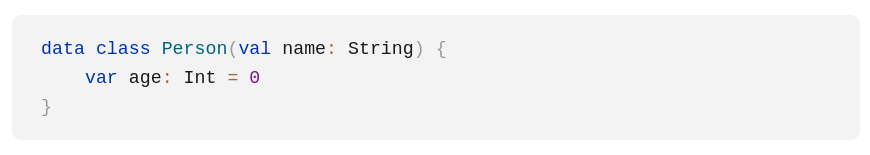
\includegraphics[width=\linewidth]{images/Dataclass.png}
\end{figure}
\end{frame}

\begin{frame}
\frametitle{Null-Sicherheit}
\begin{itemize}
    \item Safe Calls
    \item Elvis-Operator
\end{itemize}
\begin{figure}[!htb]
    \centering
    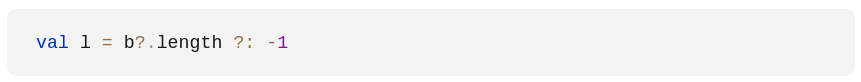
\includegraphics[width=\linewidth]{images/Elvis_operator.png}
\end{figure}

\end{frame}

\begin{frame}
\frametitle{Coroutines}
\begin{itemize}
    \item Coroutines erlauben es effizient laufende asynchrone Programme zu schreiben
    \item können als eine Art ressourcenschonender Thread gesehen werden
    \item sie werden innerhalb eines Threads ausgeführt und besitzen ihren eigenen Kontext
    \item lassen sich mit suspendierenden Funktionen anhalten
    \item sind unabhängig von einem Thread
\end{itemize}
\end{frame}


\begin{frame}
\frametitle{Infrastruktur}
\begin{itemize}
\onehalfspacing
    \item Buildsystem: Gradle, Maven
    \item Dokumentation: KDoc (analog zu JavaDoc)
    \item Entwicklungsumgebung: IntelliJ, Android Studio, Eclipse
    \item Java to Kotlin converter (J2K), konvertiert automatisch Java Klassen zu Kotlin Dateien
    \item IntelliJ Profiler, als Werkzeug zur Optimierung von Speichernutzung und Laufzeit eines Programms
\end{itemize}
\end{frame}

\begin{frame}
\frametitle{Anwendungsbereiche}
\begin{itemize}
\onehalfspacingy
    \item Android App Entwicklung: von Google empfohlene Programmiersprache
    \item Desktop- und serverbasierte Anwendungen
    \item Multiplatform (Android und iOS)
    \item Data Science und Machine Learning (kotlindl)
\end{itemize}
\end{frame}

\begin{frame}
\frametitle{Bekannte Projekte}
\begin{itemize}
\onehalfspacing
    \item Google Home, Duolingo Android App
    \item Umstieg von Java zu Kotlin
    \item verbesserte Wartbarkeit und deutliche Reduzierung der Codezeilen
\end{itemize}
\end{frame}

\begin{frame}
\frametitle{Implementierung}
\begin{itemize}
\onehalfspacing
    \item \textbf{rekursive Dateisuche:}
    \begin{itemize}
        \item existierende Java Bibliotheken enthalten hilfreiche Kotlin-Extension Funktionen (isRegularFile(), isDirectory())
    \end{itemize}
    \item \textbf{Erkennen von Binärdateien:}
    \begin{itemize}
        \item Binärdateien habe typischerweise vermehrt Steuerzeichen und ASCII Zeichen aus dem Erweiterten ASCII Zeichen Satz
        \item Algorithmus nimmt 1024 Bytes einer Datei und zählt die typischen und untypische ASCII Zeichen
        \item falls über 50\% typische ASCII Zeichen sind, wird die Datei als Binärdatei betrachtet
    \end{itemize}
    \item \textbf{Suchen von regulären Ausrücken:}
    \begin{itemize}
        \item vereinfachte Iteration durch die Textzeilen einer Datei mithilfe von Higher-Order Extension Funktionen
    \end{itemize}
\end{itemize}
\end{frame}

\begin{frame}
\frametitle{}
{\Large \centering Vielen Dank für Ihre Aufmerksamkeit!\par}
\end{frame}

\end{document}
